\chapter{FREEFLOW}
\label{ff}
% Rewrite this.
Freeflow is an instance of a virtual networking device that provides full programmability over the two major components of a network switch, the control and data planes. 

\begin{figure}[h]
\centering
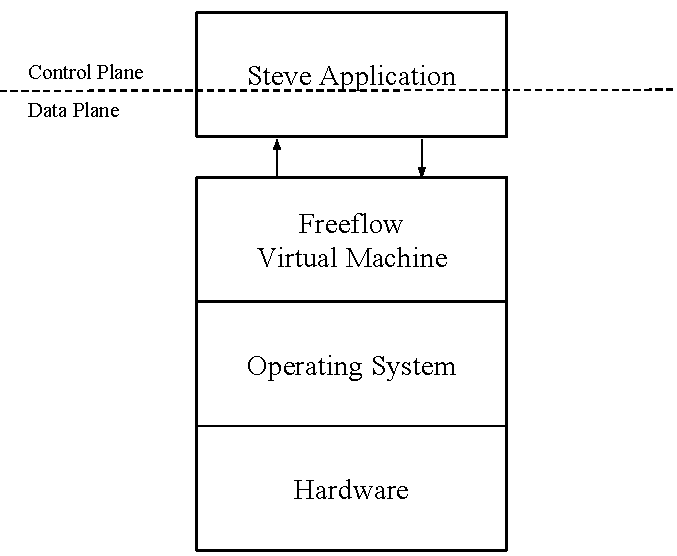
\includegraphics[scale=0.5]{ff_arch}
\caption{The Freeflow System Architecture.}
\label{ff_arch}
\end{figure}

\section{Control Plane}
\label{ff:cp}
Describe the control plane better.

\section{Data Plane}
\label{ff:dp}
Describe the data plane better.

\section{Applications}
\label{ff:app}
Describe freeflow applications.

\section{Virtual Machine}
\label{vm}
Describe the virtual machine implementation.

\begin{figure}[h]
\centering
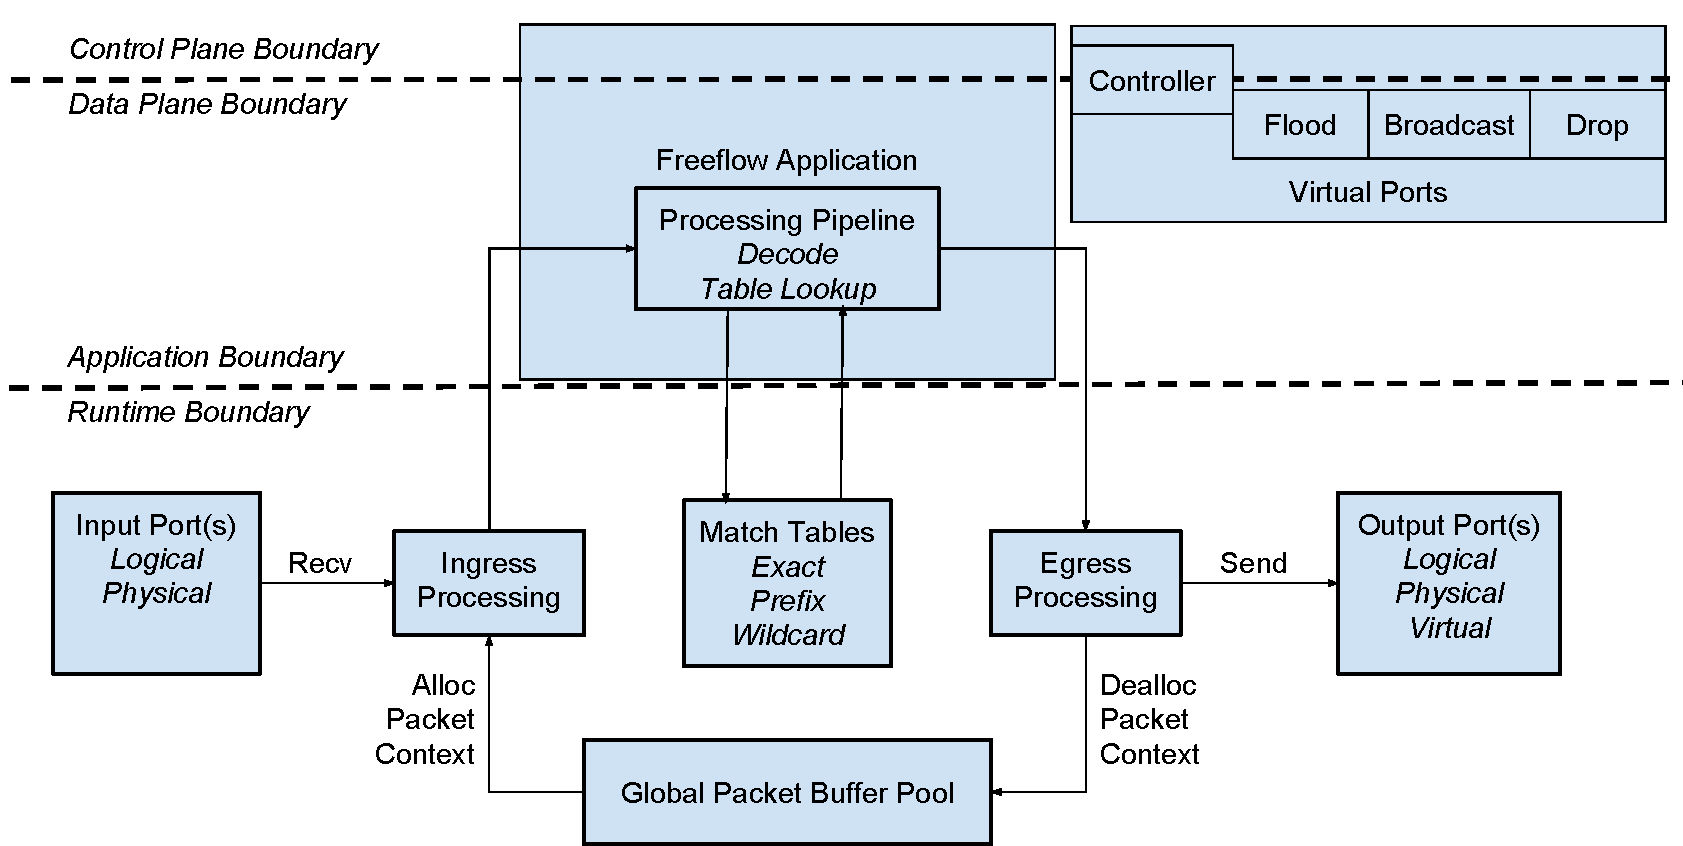
\includegraphics[scale=0.5]{ff_system}
\caption{The Virtual Machine System Architecture}
\label{fig:ff_system}
\end{figure}

\section{Ports}
\label{vm:port}
Talk about ports.

\begin{figure}[h]
\centering
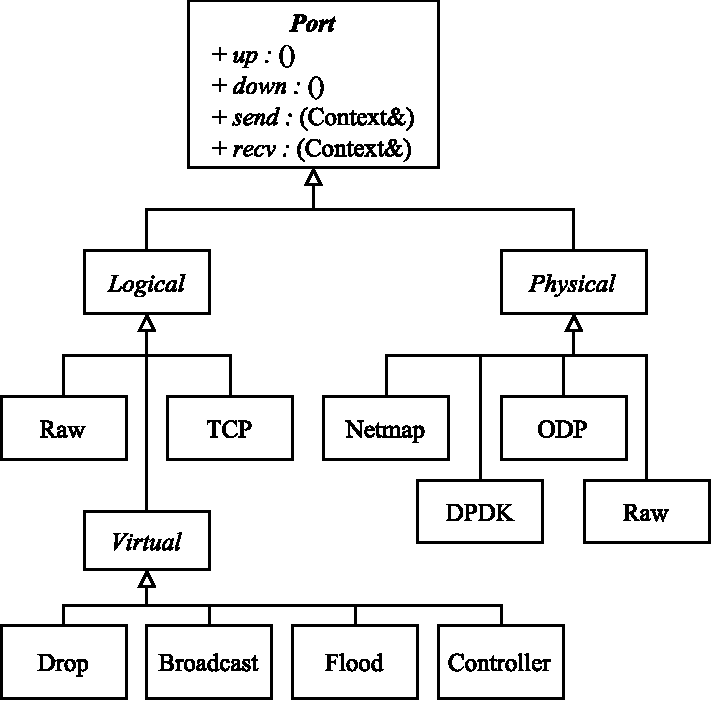
\includegraphics[scale=0.5]{ff_port_uml}
\caption{Freeflow port uml diagaram.}
\label{port_uml}
\end{figure}

\section{Tables}
\label{vm:tables}
Describe how tables are allocated and used.

\section{Packet Context}
\label{vm:context}
Lots to talk about here.

\section{Instructions}
\label{vm:insn}
Native insn execution. Offloading, optimizations.

\section{Memory}
\label{vm:memory}
Memory model.

\section{Threading}
\label{vm:threading}
Threading models.
